\chapter{Estimation de la planification}

Afin de mener à bien le projet, celui-ci est divisé en plusieurs étapes correspondant aux trois phases énoncées précédemment.  Ainsi, le diagramme de planification (figure \ref{useCase}) du projet est articulé autour de trois prototypes intégrant chacun une phase supplémentaire. 

Avant de commencer le travail sur le premier prototype, il est nécessaire de passer par une phase de modélisation et de conception (colorée en violet sur le diagramme de Gantt ci-dessous) de l'application.
Le premier prototype intègre la première phase, correspondant à la mise en place de l'algorithme d'affectation automatique des élèves ainsi que de l'outil permettant aux élèves de faire leurs choix. Sur le diagramme, les étapes nécessaires à ce prototype sont colorées en verts.

Le second prototype intégrera la phase 1 et la phase 2 du projet, c'est-à-dire la création des différents documents nécessaires au départ de l'élève. C'est aussi dans ce prototype que nous intégrerons les différents départements, rendant ainsi l'application plus générique. Comme on peut le voir sur le diagramme, les étapes (colorées en bleu) pour le prototype 2 commenceront avant la fin du premier prototype. Ce, afin de profiter de la présence de tous les membres de l'équipe.

Le troisième prototype intégrera en plus la phase 3 (colorée en jaune), ce qui signifie que ce prototype se rapprochera beaucoup de la version finale du projet. Avec ce prototype, le suivi des élèves sera mis en place.
Enfin, une dernière période servira à la rectification du troisième prototype, à l'ajout d'une interface plus ergonomique et aux derniers réglages de l'application avant la mise en production de la version finale. 

\begin{figure}[!h]
  \centering
  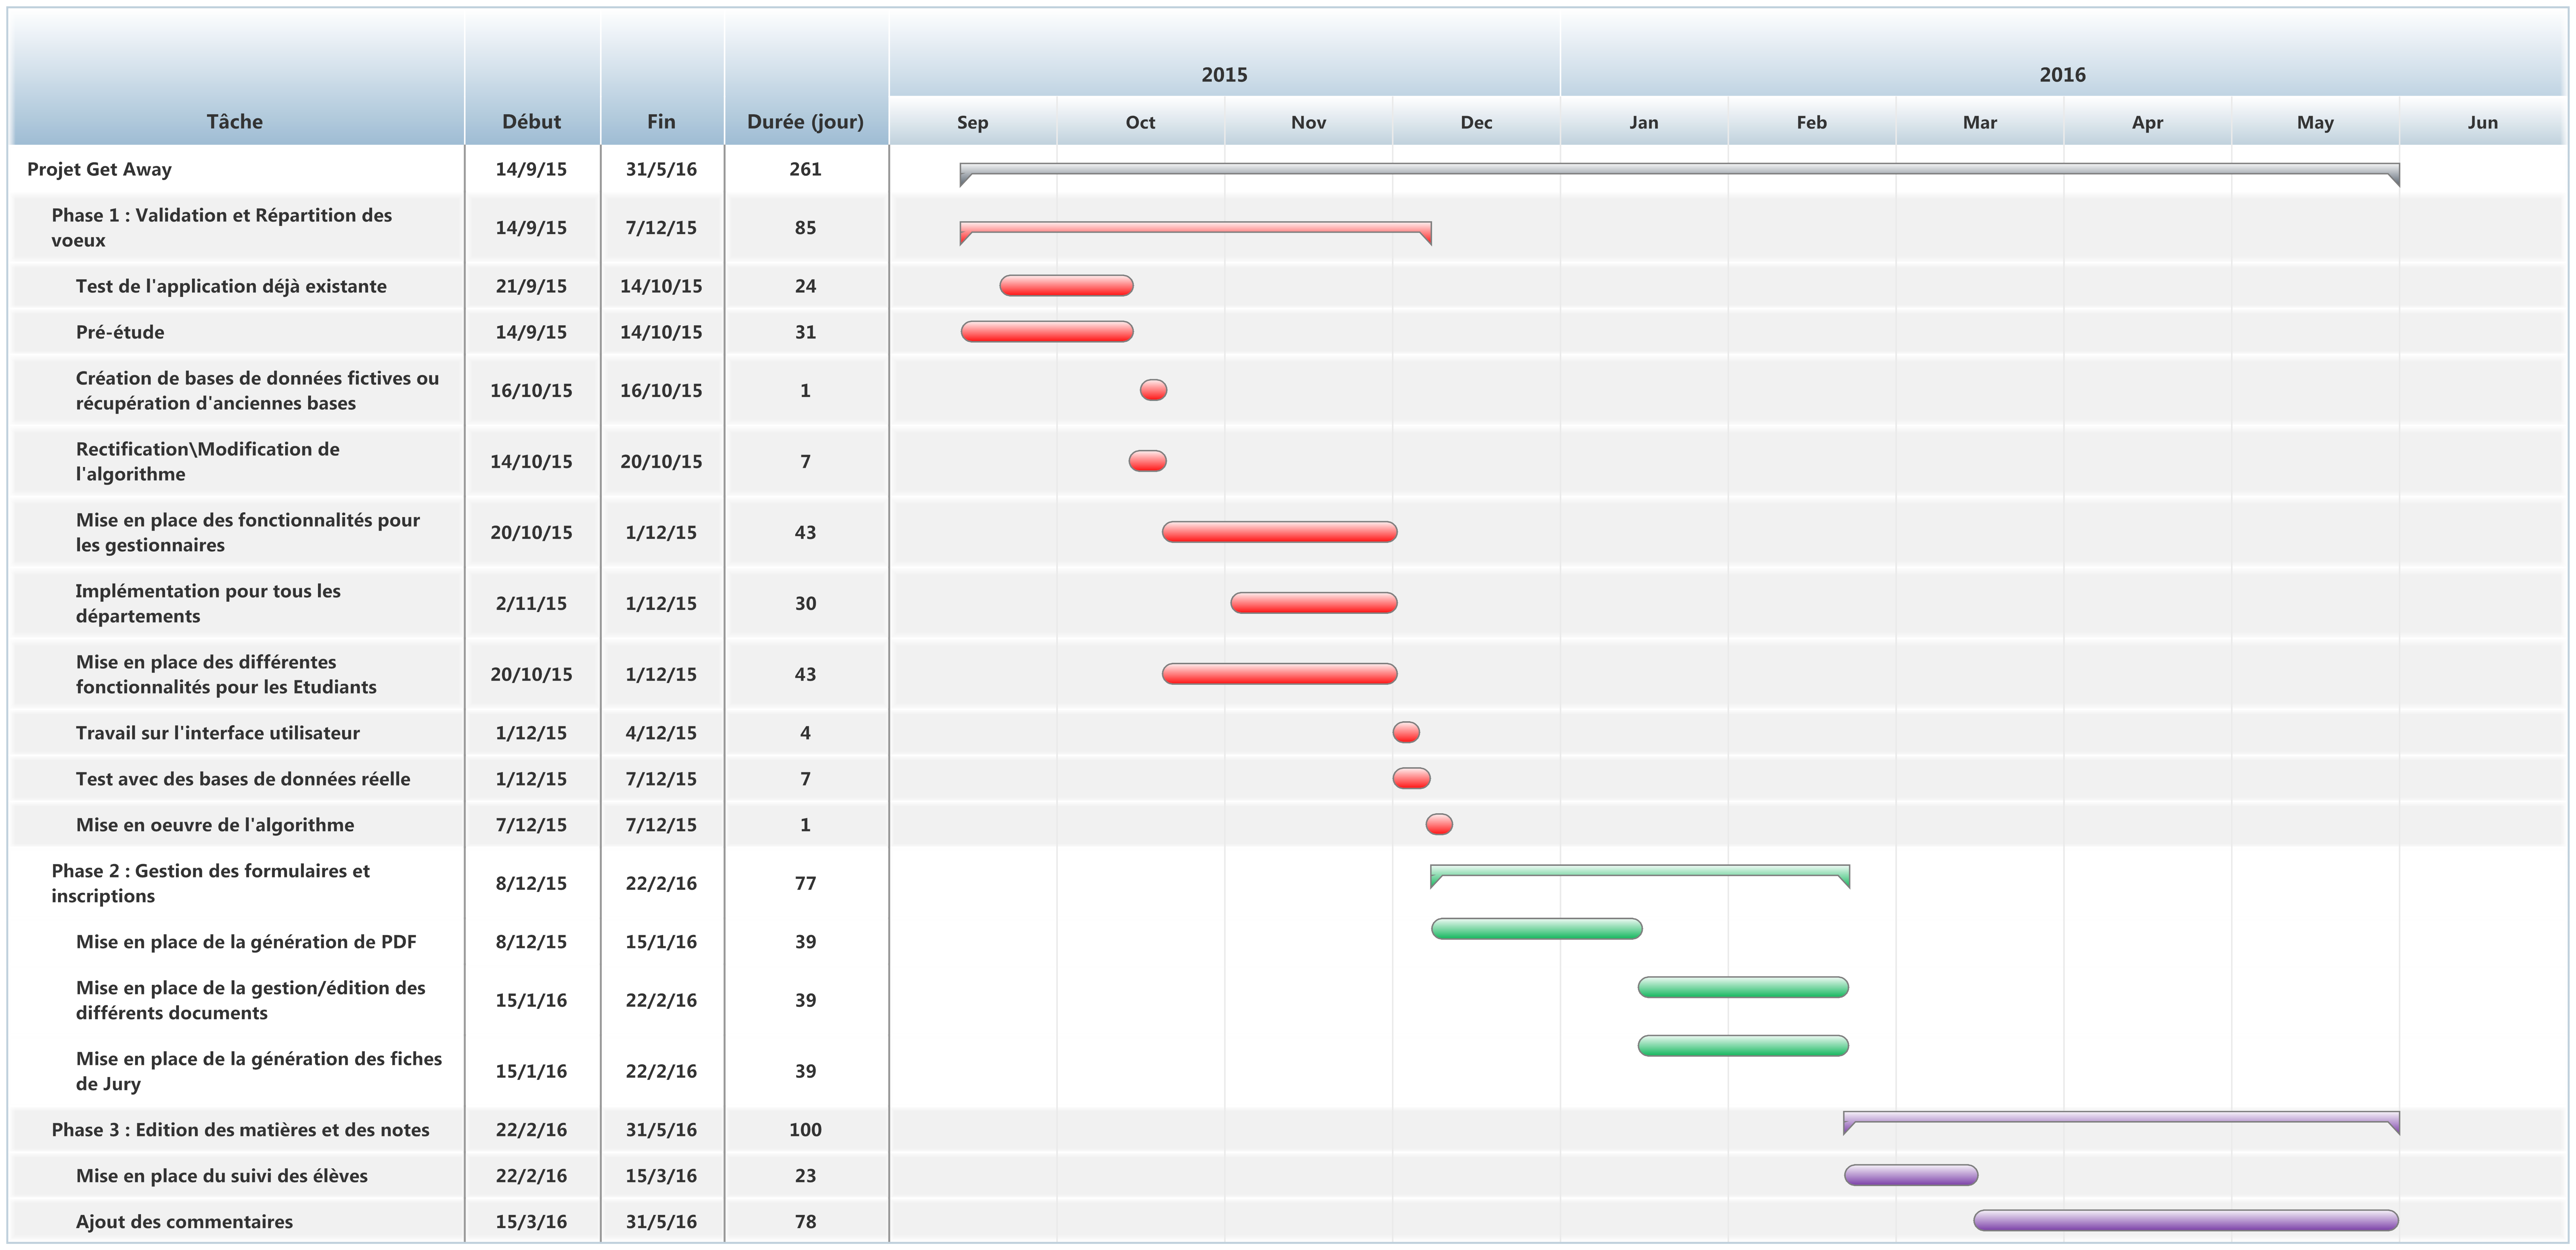
\includegraphics[angle=90, height=19cm]{Plannification/Projet.png}
  \caption{Diagramme de Gantt}
  \label{useCase}
\end{figure}